\section{ボタン押し課題のシステム}
\subsection{システム構成}
本研究で行う客観評価による調査では,被験者が行う課題にボタン押し課題を採用する.
この調査で採用するボタン押し課題は,遅延聴覚フィードバックの下で,一定の時間間隔でボタンを押下する課題を行うというものである.
このボタン押し課題を使用して,遅延聴覚フィードバックが身体運動に与える影響を様々な年代の被験者について調査することができる.
被験者がボタンを押す間隔を記録し,遅延を加えることでそのばらつきがどのように変化するかを調査する.
この方法により,遅延聴覚フィードバックが身体運動に与える影響を客観的に評価することが可能になる.
また,馴化による効果を考慮するため,ボタンの押下回数が4の倍数に到達したときのみ,聴覚フィードバックの遅延を発生させる.
% この課題を行うために,被験者が使用するシステムの構成を図\ref{fig:button-click-system}に示す.
% \begin{figure}[tb]
%   \centering
%   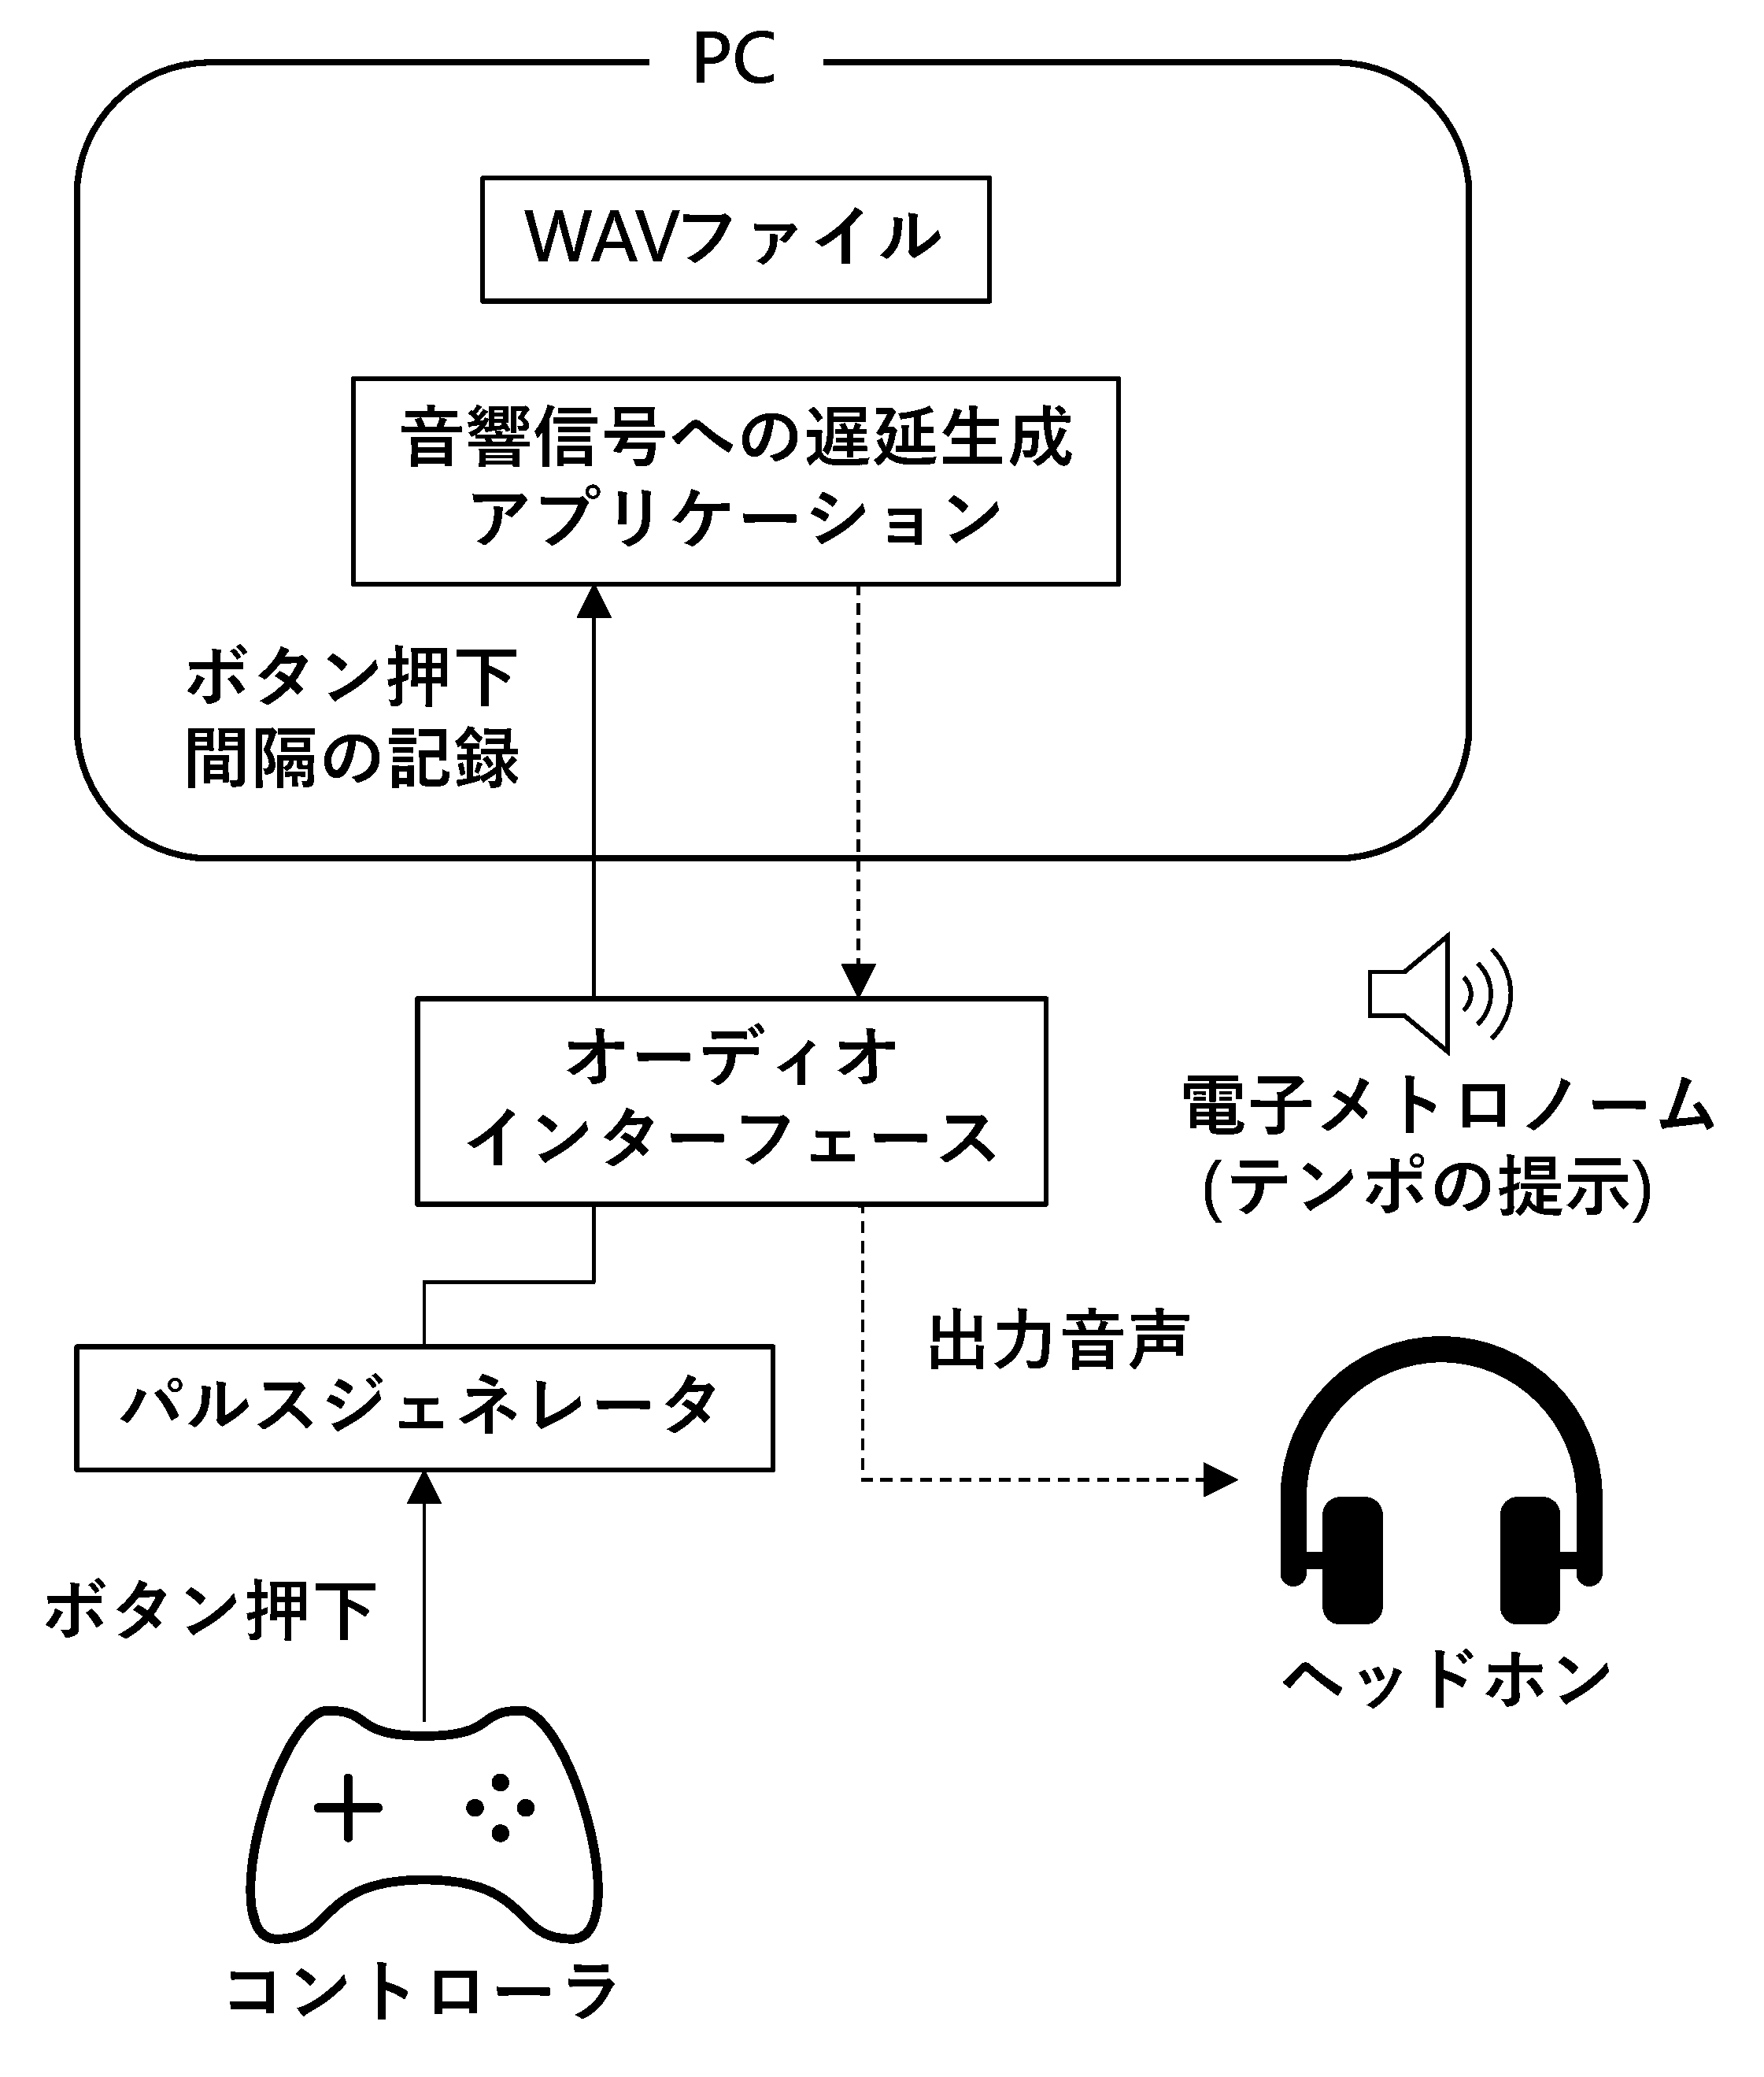
\includegraphics[scale=0.15]{figures/system_button_click.pdf}
%   \caption{調査システムの構成}
%   \label{fig:button-click-system}
% \end{figure}